\RequirePackage[l2tabu,orthodox]{nag}
\documentclass[11pt,letterpaper]{article}
\usepackage[T1]{fontenc}
\usepackage[utf8]{inputenc}
\usepackage{crimson}
\usepackage{helvet}
\usepackage[strict,autostyle]{csquotes}
\usepackage[USenglish]{babel}
\usepackage{microtype}
\usepackage{authblk}
\usepackage{booktabs}
\usepackage{caption}
\usepackage{endnotes}
\usepackage{geometry}
\usepackage{graphicx}
\usepackage{hyperref}
\usepackage{natbib}
\usepackage{rotating}
\usepackage{setspace}
\usepackage{titlesec}
\usepackage{url}
\usepackage{soul}
\usepackage[dvipsnames]{xcolor}
\usepackage[many]{tcolorbox}
\newtcolorbox{mybox}{colback = black!5!gray!50, colframe = black!75!black, segmentation style={solid}} % create text box
\usepackage{hanging}

% location of figure files, via graphicx package
\graphicspath{{./figures/}}

% configure the page layout, via geometry package
\geometry{
	paper=letterpaper,
	top=4cm,
	bottom=4cm,
	left=4cm,
	right=4cm}
\setstretch{1.02}
\clubpenalty=10000
\widowpenalty=10000

% set section/subsection headings as the sans serif font
\titleformat{\section}{\normalfont\sffamily\large\bfseries}{\thesection.}{0.3em}{}
\titleformat{\subsection}{\normalfont\sffamily\small\bfseries}{\thesubsection.}{0.3em}{}

% make figure/table captions sans-serif small font
\captionsetup{font={footnotesize,sf},labelfont=bf,labelsep=period}

% configure pdf metadata and link handling
\hypersetup{
	pdfauthor={Francisco Rowe, Robin Lovelace, Adam Dennett},
	pdftitle={Spatial Interaction Modelling: A Manifesto},
	pdfsubject={Spatial Interaction Modelling: A Manifesto},
	pdfkeywords={Spatial interaction modelling, Gravity modelling, Machine learning, Geographic data science},
	pdffitwindow=true,
	breaklinks=true,
	colorlinks=false,
	pdfborder={0 0 0}}

\title{Spatial Interaction Modelling: A Manifesto\footnote{\textbf{Citation}: Rowe, F. Lovelace, R. Dennett, A., 2022. Spatial Interaction Modelling: A Manifesto. In: Wolf, L., Heppenstall, A., and Harris, R. (eds) Edward Elgar Books}}
\author[1]{Francisco Rowe \thanks{\textit{Email}: F.Rowe-Gonzalez@liverpool.ac.uk}}
\affil[1]{Geographic Data Science Lab, Department of Geography and Planning, University of Liverpool, Liverpool, United Kingdom}
\author[2]{Robin Lovelace \thanks{\textit{Email}: R.Lovelace@leeds.ac.uk}}
\affil[2]{Institute for Transport Studies, University of Leeds, Leeds, United Kingdom}
\author[3]{Adam Dennett \thanks{\textit{Email}: a.dennet@ucl.ac.uk}}
\affil[3]{The Bartlett Centre for Advanced Spatial Analytics, University College London, London, United Kingdom}

\date{}

% From pandoc:
% https://github.com/jgm/pandoc-templates/blob/master/default.latex
\newlength{\cslhangindent}
\setlength{\cslhangindent}{1.5em}
\newlength{\csllabelwidth}
\setlength{\csllabelwidth}{3em}
\newlength{\cslentryspacingunit} % times entry-spacing
\setlength{\cslentryspacingunit}{\parskip}
\newenvironment{CSLReferences}[2] % #1 hanging-ident, #2 entry spacing
 {% don't indent paragraphs
  \setlength{\parindent}{0pt}
  % turn on hanging indent if param 1 is 1
  \ifodd #1
  \let\oldpar\par
  \def\par{\hangindent=\cslhangindent\oldpar}
  \fi
  % set entry spacing
  \setlength{\parskip}{#2\cslentryspacingunit}
 }%
 {}
\usepackage{calc}
\newcommand{\CSLBlock}[1]{#1\hfill\break}
\newcommand{\CSLLeftMargin}[1]{\parbox[t]{\csllabelwidth}{#1}}
\newcommand{\CSLRightInline}[1]{\parbox[t]{\linewidth - \csllabelwidth}{#1}\break}
\newcommand{\CSLIndent}[1]{\hspace{\cslhangindent}#1}
\setlength{\emergencystretch}{3em} % prevent overfull lines
\providecommand{\tightlist}{%
  \setlength{\itemsep}{0pt}\setlength{\parskip}{0pt}}

% https://stackoverflow.com/questions/41052687/rstudio-pdf-knit-fails-with-environment-shaded-undefined-error
\usepackage{color}
\usepackage{fancyvrb}
\newcommand{\VerbBar}{|}
\newcommand{\VERB}{\Verb[commandchars=\\\{\}]}
\DefineVerbatimEnvironment{Highlighting}{Verbatim}{commandchars=\\\{\}}
% Add ',fontsize=\small' for more characters per line
\usepackage{framed}
\definecolor{shadecolor}{RGB}{248,248,248}
\newenvironment{Shaded}{\begin{snugshade}}{\end{snugshade}}
\newcommand{\AlertTok}[1]{\textcolor[rgb]{0.94,0.16,0.16}{#1}}
\newcommand{\AnnotationTok}[1]{\textcolor[rgb]{0.56,0.35,0.01}{\textbf{\textit{#1}}}}
\newcommand{\AttributeTok}[1]{\textcolor[rgb]{0.77,0.63,0.00}{#1}}
\newcommand{\BaseNTok}[1]{\textcolor[rgb]{0.00,0.00,0.81}{#1}}
\newcommand{\BuiltInTok}[1]{#1}
\newcommand{\CharTok}[1]{\textcolor[rgb]{0.31,0.60,0.02}{#1}}
\newcommand{\CommentTok}[1]{\textcolor[rgb]{0.56,0.35,0.01}{\textit{#1}}}
\newcommand{\CommentVarTok}[1]{\textcolor[rgb]{0.56,0.35,0.01}{\textbf{\textit{#1}}}}
\newcommand{\ConstantTok}[1]{\textcolor[rgb]{0.00,0.00,0.00}{#1}}
\newcommand{\ControlFlowTok}[1]{\textcolor[rgb]{0.13,0.29,0.53}{\textbf{#1}}}
\newcommand{\DataTypeTok}[1]{\textcolor[rgb]{0.13,0.29,0.53}{#1}}
\newcommand{\DecValTok}[1]{\textcolor[rgb]{0.00,0.00,0.81}{#1}}
\newcommand{\DocumentationTok}[1]{\textcolor[rgb]{0.56,0.35,0.01}{\textbf{\textit{#1}}}}
\newcommand{\ErrorTok}[1]{\textcolor[rgb]{0.64,0.00,0.00}{\textbf{#1}}}
\newcommand{\ExtensionTok}[1]{#1}
\newcommand{\FloatTok}[1]{\textcolor[rgb]{0.00,0.00,0.81}{#1}}
\newcommand{\FunctionTok}[1]{\textcolor[rgb]{0.00,0.00,0.00}{#1}}
\newcommand{\ImportTok}[1]{#1}
\newcommand{\InformationTok}[1]{\textcolor[rgb]{0.56,0.35,0.01}{\textbf{\textit{#1}}}}
\newcommand{\KeywordTok}[1]{\textcolor[rgb]{0.13,0.29,0.53}{\textbf{#1}}}
\newcommand{\NormalTok}[1]{#1}
\newcommand{\OperatorTok}[1]{\textcolor[rgb]{0.81,0.36,0.00}{\textbf{#1}}}
\newcommand{\OtherTok}[1]{\textcolor[rgb]{0.56,0.35,0.01}{#1}}
\newcommand{\PreprocessorTok}[1]{\textcolor[rgb]{0.56,0.35,0.01}{\textit{#1}}}
\newcommand{\RegionMarkerTok}[1]{#1}
\newcommand{\SpecialCharTok}[1]{\textcolor[rgb]{0.00,0.00,0.00}{#1}}
\newcommand{\SpecialStringTok}[1]{\textcolor[rgb]{0.31,0.60,0.02}{#1}}
\newcommand{\StringTok}[1]{\textcolor[rgb]{0.31,0.60,0.02}{#1}}
\newcommand{\VariableTok}[1]{\textcolor[rgb]{0.00,0.00,0.00}{#1}}
\newcommand{\VerbatimStringTok}[1]{\textcolor[rgb]{0.31,0.60,0.02}{#1}}
\newcommand{\WarningTok}[1]{\textcolor[rgb]{0.56,0.35,0.01}{\textbf{\textit{#1}}}}


\begin{document}

\maketitle



\begin{abstract}

Spatial interaction models (SIMs) are a core tool in spatial data modelling to predict spatial flows and understand their underpinning factors. 
SIMs have been applied to provide data insights and support decision making in multiple settings, notably in transport, human mobility, migration and epidemiology. 
While considerable progress has been made on advancing the theoretical and methodological underpinnings of SIMs, key challenges remain to facilitate the application of SIMs, extend existing modelling approaches, and leverage the opportunities afforded by Big Data.
We identify three key challenges: reproducibility, calibration and Big Data modelling. 
We propose a blueprint to tackle these challenges by identifying four areas of development: 
(1) to enable essential infrastructure to facilitate the training, calibration and reproducibility of SIMs; 
(2) to embrace modelling frameworks to capture spatial, temporal and population heterogeneity; 
(3) to enhance statistical inference to accommodate Big Data analysis; and, 
(4) to integrate data science approaches to enhance SIM-generated predictions and statistical inference

%\vspace{1cm}
\end{abstract}



\pagebreak

\hypertarget{definition-and-uses}{%
\section{Definition and Uses}\label{definition-and-uses}}

For over 70 years, spatial interaction models (SIMs) have been a key tool to simulate flows between entities at different locations in physical space.
SIMs represent mathematical formulations through which the spatial interaction between geographic places encoded in aggregate flows of people, information and goods can be rendered.
Intuitively, these models seek to represent the spatial interaction between places as a function of three components: origin characteristics, destination characteristics and the separation between origins and destinations.
Originally adapted from physics, spatial flows between an origin and a destination were conceived to be proportional to their gravitational force and inversely related to their spatial separation.
Characteristics of origins and destinations are used to represent gravitational forces pushing and/or pulling people, information and goods from and to specific locations, and different forms of distance and costs are used to represent the deterring effects of geographical separation on spatial flows.

SIMs have been applied in a wide range of contexts to support data analysis and decision making in retail, transport, housing, epidemiology, public health, land use, urban and population modelling and planning projection and forecasting contexts.
SIMs are generally used for two key purposes: prediction and inference.
The \emph{prediction} of the size and direction of spatial flows has been used to predict the impact of new service units, such as shopping stores, healthcare facilities and housing units on the potential demand for associated services and traffic patterns (e.g. Fotheringham and O'Kelly 1989). Predictions from such analyses enable the identification of optimal locations and size for potential new service units. A second key purpose of SIMs is \emph{inference} about the factors shaping the spatial interactions in a network of flows. SIMs have been used to determine and understand the influence of retail store on consumers' store choices and place attributes on migration decisions and commuting patterns (e.g. Rowe et al. 2022). SIMs have also been used to delineate geographical areas of service and retail catchment areas (e.g. Reilly 1929).

SIMs take a range of forms.
Gravity models are probably the most widely known and used form of spatial interaction models in social sciences.
Adapted from physics, the basic gravity model assumes that the interactions \(T_{i j}\) between an origin \(i\) and a destination \(j\) in the form of flows can be understood as a function of driving forces like masses \(V_{i}\) and \(W_{j}\) , and a measure of spatial separation \(c_{ij}\) .
Areas are assumed to interact in a positively reinforcing way that is multiplicative of their masses, and at the same time their interactions are expected to diminish with the intervening role of spatial separation.
Spatial separation is generally measured by distance, cost or time involved in the interaction, and is often represented by a distance-decay function.
In human systems the model generally also incorporates a constant (typically called \(k\)) ensuring that expected flows do not exceed observed totals, and \(\beta\) parameter representing the deterring effect of spatial separation, or distance.
The key task in a gravity model is to estimate these parameters (i.e.~\(k\) and \(\beta\) ).
A typical notation for the model is:

\[
T_{i j}=k \frac{V_{i} W_{j}}{c_{i j}^{\beta}}
\]

In practice, a matrix of flows, between a set of origins, a set of destinations and a measure of spatial separation between origins and destinations, is the key input for SIMs.
A family of SIMs encapsulating four distinctive shapes is typically considered (Wilson 1971).
An \emph{unconstrained} formulation of the model is actually constrained to ensure that the total sum of the predicted flows from a gravity model be equal the total sum of the observed flows across all origins and destinations.
\emph{Constrained} versions are used to ensure that specific origin or destination observations are met.
Three general formulations of constrained models are used: production-constrained, attraction-constrained and doubly constrained models.
\emph{Production-constrained} forms are used to constrain a model so that the predicted number of trips emanating from each origin is equal to the observed number of trips.
\emph{Attraction-constrained} forms do the same but at the destination.
\emph{Doubly constrained} models combine these two sets of constraints.

SIMs have been extended in six key ways.
First, social science theory has been infused to underpin and enrich SIMs.
SIMs were originally conceptualised as a mathematical formulation to represent observed relationships between origins and destinations encoded in a origin-destination matrix, and generate accurate prediction of spatial flows.
Field-specific theories have been used to extend and develop the fundamental structure of SIMs to understand retail, trade, transport, communication, migration and mobility patterns.
Second, more sophisticated measures to capture the influence of origins and destinations have been developed.
The specification of SIMs has moved away from relying on population size to approximate the propulsive effect of origins and attractive force of destinations, to capture local economic, political, cultural and social differences across origins and destination, and recognise propulsive and attractive effects at play in both origins and destinations.
Third, measures of spatial separation have been refined to more appropriately reflect the geographical, psychological and financial distance and costs between origins and destinations (Schwartz 1973). Route distances on road networks are easier to compute via routing engines and interfaces Morgan et al. (2019) and distances between human settlements can be more precisely estimated based on satellite imagery (Niedomysl et al. 2017).
Fourth, considerable methodological work has been done to conceptualise and operationalise the influence of spatial structure in SIMs (Oshan 2021).
Five generalisable approaches have been proposed to account for spatial structure in distinctive ways: competing destination models by including an accessibility measure (Fotheringham 1983); Box--Cox transformations by using a Box--Cox functional form of distance (Tiefelsdorf 2003); spatial choice modelling by accounting for destination alternative substitution patterns (Hunt, Boots, and Kanaroglou 2004); spatial econometric modelling (LeSage and Pace 2008) and eigenvector spatial filtering (Chun and Griffith 2011) by incorporating spatial dependence or spatial autocorrelation.
Fifth, frameworks to calibrate SIMs have evolved.
Early methods of calibration comprised linear programming and non-linear optimization.
Regression methods have now become prominent evolving from linear log-normal model formulations using ordinary least squares (OLS) and maximum likelihood estimation procedures, through generalised linear frameworks using iteratively reweighted least squares (IWLS), especially Poisson and Negative Binomial distributions (Flowerdew and Aitkin 1982), to more sophisticated multilevel and discrete choice models to capture origin-, destination- or origin-destination-specific parameters (Davies, Greenwood, and Li 2001).
Sixth, alternative frameworks of spatial interaction modelling have been developed to incorporate different ways of conceptualising the decision-making process of choosing a destination location.
The radiation (Simini et al. 2012), exploration and preferential return (Pappalardo et al. 2015) and random utility models (McFadden 1974) have become prominent frameworks to model spatial flows, particularly human mobility flows.

Thus, considerable progress has been made on advancing the theoretical and methodological underpinnings of SIMs.
Yet, major challenges remain in terms of reproducibility, calibration and \emph{Big Data} modelling.
We believe that addressing these challenges are key to facilitate the application of SIMs, extend existing modelling approaches, leverage the greater geographical and temporal breadth, depth, scale and timeliness of \emph{Big Data} and ultimately enhance our understanding human interactions and our social world.

\hypertarget{challenges}{%
\section{Challenges}\label{challenges}}

In this section, we describe why the areas identified above are seen as key challenges.

\hypertarget{reproducibility}{%
\subsection{Reproducibility}\label{reproducibility}}

Reproducibility of SIMs has not been a prominent area of attention in past research.
Replicating most SIM applications would certainly be a challenge.
Such situation is unfortunate as this may have limited the applicability and portability of sophisticated frameworks to estimate SIMs and capture the effects of spatial structure on spatial flows.
In fact, many sophisticated SIMs have been developed to capture the effects of spatial structure on spatial flows, but the accessibility and applicability of such models remained limited.
Arguably even the application of basic formulations of SIMs tends to represent a daunting challenge for beginning modelers of spatial flow data.
The lack of reproducibility as a standard research practice has tended to generate ``black box'' data analyses, preventing the validation, verification and comparability of SIM estimates.

Understandably, reproducibility was not a concern during the 1970s and 1980s, when significant progress was made on developing SIMs.
Computer hardware, software and know-how needed to develop and deploy SIMs were unavailable to most people.
Even when consumer laptops became widely available and more affordable during the 2000s, few well-known user-friendly off-the-shelf options to implement SIMs existed.
Yet, today, computer software and hardware are highly affordable and learning computing programming has become increasingly accessible.
With the advent of open science, resources to learn computer programming in popular data science languages, such as \emph{R} and \emph{Python} have become widely available.
Nevertheless, most SIM applications can still not be reproduced.

Yet, reproducibility of SIM estimates can yield key benefits for future research, impact and training .
Reproducible research can boots citations and facilitate comparability of research results enabling the application of existing methods to a wide range of contexts (Brunsdon 2016).
Reproducibility can also enhance accountability, validation and verification of research findings by increasing transparency (Brunsdon 2016).
By transparently sharing open data products, including reproducible code and input data, (Arribas-Bel et al. 2021) used in the analysis, results can be validated and lessons can be learnt from the limitations and strengths of the application of particular methods.
Reproducible open products can also increase the portability of existing work.
New research can build on existing code and data focusing on addressing novel questions, and avoiding reinvention of wheels.
Reproducible work can facilitate the generation of updates as new data become available.
Reproducible open data products can also be used as communication and impact strategy expanding the original purpose of research findings (Nüst and Pebesma 2021).
Reproducible code and data can be used to provide educational training and enable practitioners to address policy questions which were not outside the scope of the original research project (Rowe et al. 2020).

\hypertarget{calibration}{%
\subsection{Calibration}\label{calibration}}

Calibration is at the centre of what makes spatial interaction models useful to researchers and practitioners.
As Openshaw (1975) describes it, ``calibration is the process of providing estimates of the unknown parameters we have identified as the independent variables of the model.'' In a basic gravity formulation, we seek to estimate three parameters - as identified above - relating to origin mass, destination mass and a parameter determining the frictional effect of spatial separation between origins and destinations.
These parameters reveal information about our system of interest.

Yet, we identified key challenges relating to the calibration of SIMs.
Calibration requires both data and software.
Forty or fifty years ago when many of the theoretical foundations of spatial interaction modelling were laid, the data landscape was somewhat different from today -- spatial flow data were rarely available in volume and certainly not at the sort of temporal rhythm they are now.
Supermarket loyalty-card holders generate origin/destination revenue flow data from residential origins to store destinations at daily frequencies over time periods that can cover many years or even decades.
As such, we might be forgiven for expecting that even if the science and theory underpinning the models has not developed very much, the software and processes facilitating calibration -- relating empirical observations to the theoretical representations embodied in the models -- might have.
But in many ways, they have not.
Today spatial flow data are ubiquitous.
They can be derived from digital traces collected across various sensor networks involving mobile phones, social media, loyalty cards, smart card tickets and credit cards.
Accessing interaction data is thus not the barrier it once was.

Yet, making sense of these data remains a challenge.
Much of the challenge is because there is a dearth of knowledge within geographical education.
Despite SIMs underpinning many social and geographical processes, these models are not taught to undergraduate geography students in the same way as, say, regression models are taught to economists or social psychologists.
As such, it is not immediately obvious, even for those with geography degrees, how anyone might go about fitting their spatial flow data to a theoretical model, calibrating the parameters and revealing properties of their system.
But, why have cohorts of undergraduate geography students not been taught how to fit these models and explore systems of spatial interaction?

Accessibility seems to represent an obstacle for the wider applicability of SIMs.
We discussed issues around reproducibility challenging the practical application of SIMs, but that with packages like \texttt{SPINT} (Oshan 2016) and our own efforts with the \texttt{simodels} package in \emph{R} (see Section \ref{enabling-infrastructure}), the tide is beginning to turn.
Yet, calibration remains a challenging sub-topic for reproducibility and wider accessibility of these models, particularly where algorithms which are able to calibrate parameters have remained locked away - either behind dense algebraic notation in dusty papers from the 1970s, or where they have found their way into commercial software, behind paywalls.

Ironically, effective calibration routines have been available for as long as students have been running regression models in their introductory statistics classes.
Occasional references can be found in the historic literature (e.g. Fotheringham and Webber 1980; Flowerdew and Aitkin 1982) which lift the curtain and reveal that through reformulating the classic Wilsonian entropy maximising spatial interaction model as either a logged OLS regression model or a GLM utilising Poisson or negative binomial distributions, multiple parameters can be calibrated easily.
These models are all available in common statistical software packages; but for most trying to make sense of the field coming across papers by some of the doyens (for it was and still is a male-dominated field) of the scene, practical expediency is often sacrificed at the alter of theoretical or technical prowess.
And even then, while undoubtedly mathematically and theoretically rigorous, notes on calibration can be presented either as passing reference to `least squares' or worse a lengthy derivation of maximum likelihood or Newton Raphson methods with no practical middle ground to assist novices in running a model.

\hypertarget{big-data-modelling}{%
\subsection{Big Data modelling}\label{big-data-modelling}}

As argued above, new technologies have enabled the emergence of `Big Data' through the production and storage of large volumes of digital data.
Much of these data contain location information and hence offer an opportunity to derive spatial flow data and understand spatial interactions between places.
Big Data offer unique opportunities to study spatial interactions at unprecedented detailed geographical and temporal scales in real or near real-time across extensive populations and geographical areas.
However, leveraging on these opportunities also involves major challenges for the analysis and modelling of spatial interactions (Rowe 2021).
Furthermore, Big Data sources have often analysed `as-is', without due attention paid to levels of validity and cross-comparison between data sources.
Validation techniques and model/aggregate-data comparisons can help overcome these issues (Lovelace et al. 2016).

Limited research has focused on explicitly capturing patterns of non-stationarity in spatial interaction modelling despite the availability of suitable methods (Oshan 2021).
While the issues of calibration discussed in Section \ref{calibration} may have represented a barrier, lack of large enough data sets may have also hindered progress.
Before the emergence of Big Data, the most common form of spatial flow data were cross-sections of origin-destination matrices derived from censuses or surveys, offering information at coarse geographical scales and population subgroups.
The rise of data now offers more granular and denser volumes of data to capture previously unrepresented patterns of spatial, temporal and population non-stationarity.
The adoption and adaption of more sophisticated modelling frameworks will thus be required to effectively uncover these patterns.

Big Data also represent challenges for statistical inference.
A standard practice in social sciences is to be guided by \emph{p} values.
Regression model estimates with \emph{p} values below 0.05 threshold are commonly considered statistically significant and thus these estimates take central stage in most analyses.
Modelling estimates derived from large data sets, however, often render \emph{p} values below this threshold, calling for the adoption of alternative approaches.
Such situation aligns with more general calls for a stop to the use of P values in the conventional, dichotomous way - to decide whether a result supports or refutes a scientific hypothesis.
Additionally, Big Data offer an opportunity to embrace causal inference approaches.
Reliance on cross-sectional data hindered the wide adoption of causal inference approaches to study the determinants of spatial interactions.
Big Data now provides large, detailed longitudinal data sets to track spatial interactions and establish cause-and-effect relationships.
Though, obtaining suitable time-varying data on relevant factors believed to shape the dynamics of spatial interactions may remain an obstacle.
While data may be available, spatial integration of data may not be possible because of ethical considerations and data governance issues.

New methods are also required to handle, analyse and store large data sets.
Traditional SIM frameworks were designed to identify significant relationships in small sample sizes with known properties.
Big data are not collected for research purposes.
They are an unintended consequence of administrative processes or social interactions and need to be reengineered for research (Rowe 2021) .
Handling Big Data requires a wider and new digital skills set, largely based on machine learning and artificial intelligence (ML/AI) and coding, in addition to greater knowledge of computing technology (e.g.computational notebooks, Github and Docker) as well as scalability and parallelisation approaches.
Except for a few centres, current university geography programmes and infrastructures are largely unprepared to deliver the required training.
A multidisciplinary approach is needed to integrate computational training into human geography.
ML/AI are likely to enhance prediction outcomes generated from SIMs.
The idea of using ML/AI to model spatial interactions is not new, but the application has been limited due to the lack of large data sets.
ML/AI are data hungry, requiring millions of data for effective training and validation.
The rise of data provides an opportunity to promote the wider adoption of these models.

\hypertarget{the-way-forward}{%
\section{The Way Forward}\label{the-way-forward}}

This section describes the areas which, we argue, should be developed to address the identified challenges.

\hypertarget{enabling-infrastructure}{%
\subsection{Enabling Infrastructure}\label{enabling-infrastructure}}

Developing the essential infrastructure is key to enhance the reproducibility and facilitate the calibration of SIMs.
Software, open science and digital technology are important elements to develop an ecosystem that fosters reproducible SIMs, provides adequate training and facilitates the application of SIMs.
We believe that an essential building block in this ecosystem is user-friendly, efficient, open source software.
Partly motivated by this chapter, we have developed the \texttt{simodels}\footnote{Short for spatial interaction models} \emph{R} package (Lovelace and Nowosad 2022) .
\footnote{The primary motivation was the need to develop SIMs to represent trips for non-commuting or non-school purposes in Ireland as part of a contract with Transport Infrastructure Ireland.} Below we present a reproducible example
. \texttt{simodels} enables the rapid develop of SIMs --- starting from basic geographic data sets as the key input --- in comparatively few lines of code
.

\texttt{simodels} does not just provide functions for running and calibrating SIM parameters.
It provides a framework for developing SIMs and creating new functions implementing different types of SIM and using a variety of pre-existing modelling tools in SIMs.
We aim to expand the functionality of the package building on the foundations presented below.
The first step is to install the package by entering and running the following command into the R console:

\begin{Shaded}
\begin{Highlighting}[]
\FunctionTok{install.packages}\NormalTok{(}\StringTok{"simodels"}\NormalTok{)}
\end{Highlighting}
\end{Shaded}

We will also install \texttt{tidyverse} for intuitive data processing functionality (Grolemund and Wickham 2016).
Load the packages as follows:

\begin{Shaded}
\begin{Highlighting}[]
\FunctionTok{install.packages}\NormalTok{(}\StringTok{"tidyverse"}\NormalTok{)}
\end{Highlighting}
\end{Shaded}

\begin{Shaded}
\begin{Highlighting}[]
\FunctionTok{library}\NormalTok{(simodels)}
\FunctionTok{library}\NormalTok{(tidyverse)}
\end{Highlighting}
\end{Shaded}

The starting `point' is geographic entities representing trip start, end (for `multi-partite' models) or intermediate points.
We use the word `features' --- meaning geographic vector entities (points, lines, polygons) --- with reference to the `simple features' standard defined by the Open Geospatial Consortium (2011).
Almost all SIMs use points and polygons as the basis of origins and destinations and raster datasets can be represented as simple features.
Such geographic features, and associated attributes (e.g.~a column named \texttt{population} representing the population of each administrative zone) can be imported from standard spatial vector data formats such as Shapefiles (\texttt{.shp}) GeoPackage (\texttt{.gpkg}) and GeoJSON (\texttt{.geojson}) files with the \texttt{sf} package:

\begin{Shaded}
\begin{Highlighting}[]
\NormalTok{origin\_zones }\OtherTok{=}\NormalTok{ sf}\SpecialCharTok{::}\FunctionTok{read\_sf}\NormalTok{(}\StringTok{"origin\_zones.geojson"}\NormalTok{)}
\NormalTok{destination\_points }\OtherTok{=}\NormalTok{ sf}\SpecialCharTok{::}\FunctionTok{read\_sf}\NormalTok{(}\StringTok{"destination\_points.geojson"}\NormalTok{)}
\end{Highlighting}
\end{Shaded}

The code chunk above imports two data objects:

\begin{enumerate}
\def\labelenumi{\arabic{enumi})}
\item
  A simple features object with `multipolygon' geometries representing administrative zones that constitute trip origins (\texttt{origin\_zones}).
\item
  A simple features object with `point' geometries representing two popular pubs in Leeds as trip destinations (\texttt{destination\_points}).
\end{enumerate}

Before creating SIMs representing travel to these two pubs in Leeds, we first perform some exploratory data analysis (EDA) to illustrate the input data (Beecham and Lovelace 2022):

\begin{Shaded}
\begin{Highlighting}[]
\NormalTok{origin\_zones }\SpecialCharTok{\%\textgreater{}\%} 
  \FunctionTok{ggplot}\NormalTok{() }\SpecialCharTok{+}
  \FunctionTok{geom\_histogram}\NormalTok{(}\FunctionTok{aes}\NormalTok{(}\AttributeTok{x =}\NormalTok{ to\_pubs), }\AttributeTok{binwidth =} \DecValTok{10}\NormalTok{)}
\NormalTok{origin\_zones }\SpecialCharTok{\%\textgreater{}\%} 
  \FunctionTok{ggplot}\NormalTok{() }\SpecialCharTok{+}
  \FunctionTok{geom\_sf}\NormalTok{(}\FunctionTok{aes}\NormalTok{(}\AttributeTok{fill =}\NormalTok{ to\_pubs), }\AttributeTok{alpha =} \FloatTok{0.5}\NormalTok{) }\SpecialCharTok{+}
  \FunctionTok{geom\_sf}\NormalTok{(}\AttributeTok{data =}\NormalTok{ destination\_points)}
\end{Highlighting}
\end{Shaded}

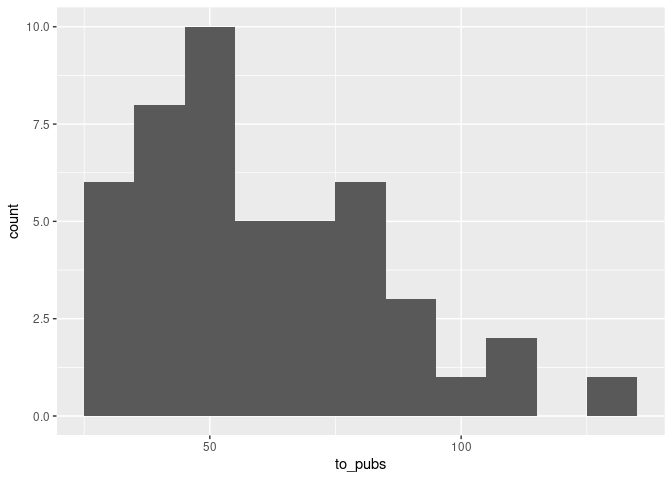
\includegraphics[width=0.5\linewidth]{README_files/figure-latex/unnamed-chunk-9-1} 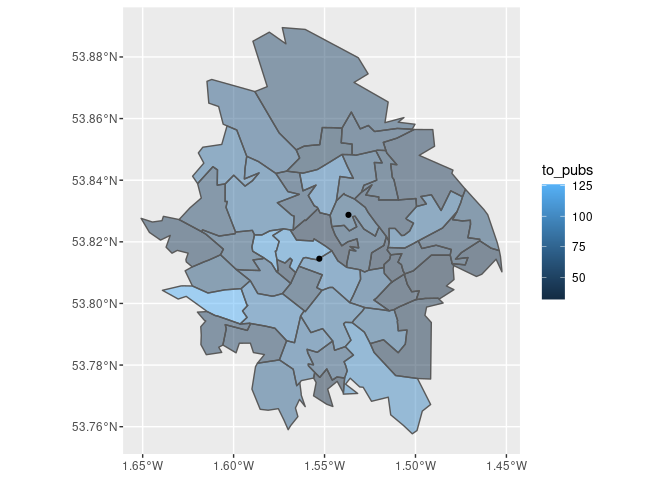
\includegraphics[width=0.5\linewidth]{README_files/figure-latex/unnamed-chunk-9-2}

For many applications, the most important function in the \texttt{simodels} package is \texttt{si\_to\_od()}:

\begin{Shaded}
\begin{Highlighting}[]
\NormalTok{od\_zones\_to\_points }\OtherTok{=} \FunctionTok{si\_to\_od}\NormalTok{(origin\_zones, destination\_points)}
\FunctionTok{class}\NormalTok{(od\_zones\_to\_points)}
\FunctionTok{nrow}\NormalTok{(od\_zones\_to\_points)}
\FunctionTok{names}\NormalTok{(od\_zones\_to\_points)}
\end{Highlighting}
\end{Shaded}

\texttt{si\_to\_od()} creates an `OD matrix' represented in long form.
As shown in the output above, the result is a data frame with 94 rows, representing the full combination of trips from each of the 47 origin zones to each of the 2 destinations.
The names in the data frame refer to variables for origin and destination locations.
When working on large input data sets, the `full matrix' of combinations can get unhelpfully large: an OD dataset from every MSOA to every pub in England, for example, would result in a data set with 350,000,000 (350 million) rows.
To reduce data set size, a `sparse matrix' representing only OD pairs below a certain distance threshold can be created by adding a \texttt{max\_dist} argument as shown below.
The maximum Euclidean distance between zone centroids and point destinations needs to be set, at 5 km in this example.
Note: \texttt{si\_to\_od()} calculates Euclidean between the full combination of origins and destinations automatically.

\begin{Shaded}
\begin{Highlighting}[]
\NormalTok{od\_zones\_to\_points }\OtherTok{=} \FunctionTok{si\_to\_od}\NormalTok{(origin\_zones, }
\NormalTok{                              destination\_points, }
                              \AttributeTok{max\_dist =} \DecValTok{5000}\NormalTok{)}
\end{Highlighting}
\end{Shaded}

The resulting origin-destination data set is smaller (79 rows compared with 94 rows previously).
While it does not lead to a major reduction in our example, the process can greatly speed-up SIM processing, modelling and visualisation run times dealing with large data sets, tackling issues outlined in Section \ref{big-data-modelling}.

We can now specify a simple SIM model as follows:

\begin{Shaded}
\begin{Highlighting}[]
\NormalTok{gravity\_model }\OtherTok{=} \ControlFlowTok{function}\NormalTok{(beta, d, m, n) \{}
\NormalTok{  m }\SpecialCharTok{*}\NormalTok{ n }\SpecialCharTok{*} \FunctionTok{exp}\NormalTok{(}\SpecialCharTok{{-}}\NormalTok{beta }\SpecialCharTok{*}\NormalTok{ d }\SpecialCharTok{/} \DecValTok{1000}\NormalTok{)}
\NormalTok{\} }
\end{Highlighting}
\end{Shaded}

and implement it with the following command:

\begin{Shaded}
\begin{Highlighting}[]
\NormalTok{od\_to\_pubs\_result }\OtherTok{=}\NormalTok{ od\_zones\_to\_points }\SpecialCharTok{\%\textgreater{}\%} 
  \FunctionTok{si\_calculate}\NormalTok{(}\AttributeTok{fun =}\NormalTok{ gravity\_model, }
               \AttributeTok{m =}\NormalTok{ origin\_to\_pubs,}
               \AttributeTok{n =}\NormalTok{ destination\_size,}
               \AttributeTok{d =}\NormalTok{ distance\_euclidean,}
               \AttributeTok{beta =} \FloatTok{0.5}\NormalTok{,}
               \AttributeTok{constraint\_production =}\NormalTok{ origin\_to\_pubs)}
\end{Highlighting}
\end{Shaded}

We can check the results:

\begin{Shaded}
\begin{Highlighting}[]
\FunctionTok{sum}\NormalTok{(od\_to\_pubs\_result}\SpecialCharTok{$}\NormalTok{interaction)}
\CommentTok{\#\textgreater{} [1] 2903}
\FunctionTok{sum}\NormalTok{(origin\_zones}\SpecialCharTok{$}\NormalTok{to\_pubs)}
\CommentTok{\#\textgreater{} [1] 2903}
\end{Highlighting}
\end{Shaded}

As shown above, the total number of trips is the same in the OD data as in the zone level data.
We can visualise the result using \texttt{ggplot} - see Figure \ref{fig:pubresmap}.

\begin{Shaded}
\begin{Highlighting}[]
\FunctionTok{library}\NormalTok{(ggspatial)}
\CommentTok{\# rosm::osm.types()}
\NormalTok{od\_to\_pubs\_result }\SpecialCharTok{\%\textgreater{}\%} 
  \FunctionTok{ggplot}\NormalTok{() }\SpecialCharTok{+}
  \FunctionTok{annotation\_map\_tile}\NormalTok{(}\AttributeTok{type =} \StringTok{"cartolight"}\NormalTok{) }\SpecialCharTok{+}
  \FunctionTok{geom\_sf}\NormalTok{(}\FunctionTok{aes}\NormalTok{(}\AttributeTok{lwd =}\NormalTok{ interaction, }\AttributeTok{colour =}\NormalTok{ D), }\AttributeTok{alpha =} \FloatTok{0.5}\NormalTok{) }\SpecialCharTok{+}
  \FunctionTok{scale\_size\_continuous}\NormalTok{(}\AttributeTok{range =} \FunctionTok{c}\NormalTok{(}\FloatTok{0.3}\NormalTok{, }\DecValTok{3}\NormalTok{)) }\SpecialCharTok{+}
  \FunctionTok{geom\_sf}\NormalTok{(}\AttributeTok{data =}\NormalTok{ origin\_zones, }\AttributeTok{fill =} \ConstantTok{NA}\NormalTok{, }\AttributeTok{lty =} \DecValTok{2}\NormalTok{, }\AttributeTok{alpha =} \FloatTok{0.5}\NormalTok{) }\SpecialCharTok{+}
  \FunctionTok{theme\_void}\NormalTok{()}
\end{Highlighting}
\end{Shaded}

\begin{figure}
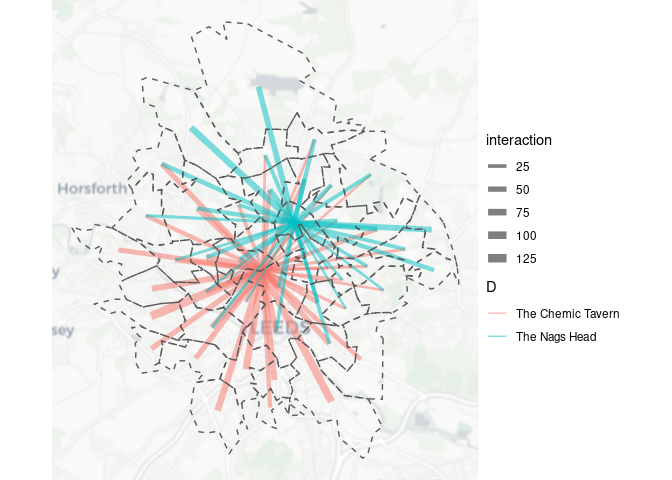
\includegraphics[width=0.8\linewidth]{README_files/figure-latex/pubresmap-1} \caption{Results of a reproducible SIM undertaken on a minimal example based on synthetic data representing hypothetical trips to 2 pubs in Leeds, UK.}\label{fig:pubresmap}
\end{figure}

\begin{verbatim}
#>   |                                                                              |                                                                      |   0%  |                                                                              |==================                                                    |  25%  |                                                                              |===================================                                   |  50%  |                                                                              |====================================================                  |  75%  |                                                                              |======================================================================| 100%
\end{verbatim}

In the future we would like to see SIM development becoming as pain-free and intuitive as possible.
We hope to see new open source SIM software projects being developed to reduce the `barrier to entry' to SIMs.
Building SIM software as part of popular languages for data science such as R, Python or Julia enables reproducibility, and access to a large ecosystem, as part of the SIM development process.

In terms of the \texttt{simodels} package briefly introduced in this section, we are at early days (the package was first published on CRAN in June 2022).
It has been tested on substantial input datasets and can certainly enable SIMs to be developed, tested, and refined rapidly.
In the future, we would like to add pre-existing SIM models, for example, a \texttt{si\_gravity()} function to provide a basic gravity model without having to specify the functional form as we did above, to the package.
Over time, we would like to implement many such functions, perhaps a step towards realising Alan Wilson's vision of a `family' of SIMs in open source software (Wilson 1971).
More broadly, the project is open source and in that spirit of collaboration will evolve organically (Franco-Bedoya et al. 2017); we encourage contributions and ideas on the project's issue tracker.\footnote{\url{https://github.com/Robinlovelace/simodels/issues}}

\hypertarget{capturing-heterogeneity}{%
\subsection{Capturing Heterogeneity}\label{capturing-heterogeneity}}

We argue that research on SIMs should seek to adopt and adapt modelling frameworks to capture and understand patterns of spatial, temporal and population non-stationarity which can now be capture given the rise of large data sets.
This line of enquiry involves calibrating models to estimate separate parameters for individual origins, destinations, time units and population segments.
Such parameters can reflect local, temporal and population variations in the relationships producing spatial flows.
Inference based on a set of global model parameters may lead to draw misleading conclusions due to misrepresentations of local-, temporal- and population-specific trends.

Yet, as noted above, limited progress has been made on capturing these patterns of non-stationarity (Oshan 2021).
Existing approaches have been proposed to capture spatial non-stationarity.
An approach involves subsetting the overall data set into origin- or destination-specific data sets and calibrate individual models for each data set.
An alternative approach is to include interaction terms between a binary categorical variable identifying an origin or destination, and each of the relevant covariates in a regression model.
A third alternative is to use geographically weighted regressions (GWRs) to capture spatial non-stationarity (Graells-Garrido et al. 2021), but the extension of these models to calibrate spatial flow count data is challenging.
It often requires the log transformation of spatial flows.
Yet, such approaches may be inappropriate when dealing with sparse origin-destination matrices containing zeros.
In such scenarios, using appropriate count distributions is recommended (O'Hara and Kotze 2010).

We propose generalised linear mixed models (GLMMs) as a more flexible modelling framework to capture all three sources of non-stationarity based on appropriate count data distributions.
GLMMs extend GLMs to incorporate a combination of random and fixed effects parameters as predictor variables, and accommodate non-continuous responses, such as binary and count responses.
Fixed effects represent a typical covariate and are typically used to capture ``global'' average patterns.
Random effects are represented by categorical variables encoding some grouping unit, and can be used to estimate the extent of variations between and within grouping units.
Random effects are flexible, and in SIMs, units could comprise groups or individual origins, destinations, origin-destination pairs, time intervals or population subgroups to capture spatial, temporal and population variations in spatial flows.
Unlike GWRs, the flexibility of GLMMs provides an opportunity to selectively capture patterns of non-stationarity in relationships with a selected group of theoretically- or policy-relevant variables.
In addition to flexibility, random effects can aid to correct statistical inference about fixed ``global'' effects by providing an estimation of variables in the response variable within and between groups.
They can also reduce the probability of Type I error and Type I error (Harrison et al. 2018).
GLMMs can also be used to explicitly model spatial and temporal auto-correlation.

Yet, challenges exist in applying GLMMs.
First, GLMMs make additional assumptions about the data to those made in standard statistical approaches and they need to be tested (Harrison et al. 2018).
Second, interpreting the model outputs from GLMMs correctly may be challenging, particularly estimates relating to variance components of random effects and correlations.
Third, model selection is a challenge because of biases in model performance tests caused by the presence of random effects (Harrison et al. 2018).
Guidelines for the implementation of GLMMs will therefore be needed to navegate these challenges and leverage the potential of these models to effectively account for non-stationarity in spatial flows.

\hypertarget{enhancing-statistical-inference}{%
\subsection{Enhancing Statistical Inference}\label{enhancing-statistical-inference}}

We argue new ways of approaching statistical inference in SIMs.
First, we call for a careful use of the concept of statistical significance.
As highlighted in Section \ref{big-data-modelling}, dichotomising estimates into `statistically significant' and `statistically non-significant' is unhelpful and can lead to draw misleading conclusions, particularly for models relying on large data sets as the full set of estimates in such models can render \emph{p} values below 0.05.
An approach is embracing uncertainty, and re-conceptualing confidence intervals as `compatibility intervals' can provide a practical solution (Amrhein, Greenland, and McShane 2019).
This shifts the focus to all values inside the interval and to the fact that emphasising a single point estimate may not be appropriate to draw broad conclusions about the factors underpinning spatial flows.

Second, we argue for greater use of causal inferential approaches.
Big Data now offers an unprecedented temporal frequency to capture spatial interactions in very short time frames, and understand the sequence of events to distinguish causes and consequences of these interactions.
Identifying these causal-effect relationships is key to understand the impact of interventions and inform the development of policies aiming at generating a desired outcome.
Inference statistical approaches are widely used in other social science disciplines, but these practices have not permeated through geography.
Causal inference on spatial processes faces additional challenges, such as spatial dependence, spatial heterogeneity and spatial effects (Akbari, Winter, and Tomko 2021).
So, while adopting causal inference methods to analyse spatial interactions may not be straightforward, we believe that it is a valuable endeavor to inform the design of future policy interventions.

Third, we propose the use of multi-model inference.
Intuitively, multi-model inference seeks to draw conclusions from a range of theoretically-sound model specifications (Burnham and Anderson 2004).
It uses model averaging to determine the direction and strength of regression predictors, and enables the generation of Akaike Information Criterion based weights from multiple models to assess the relative importance of predictors in an outcome.
As such, inferences are not drawn from a single model, leading to more robust inferences, and offers an alternative approach to evaluate the importance of predictors that does not depend on statistical significance dichotomy.
Additionally determining the relevance of factors shaping spatial flows based on multi-model inference offers an additional alternative to make inference in the context of SIMs and Big Data.
Multi-model inference has been rarely applied to capture spatial interactions (Rowe 2013).
Yet, it is widely used in biology and ecology, and various routines exist in \emph{R} which can be integrated with \texttt{simodels}.

\hypertarget{integrating-data-science}{%
\subsection{Integrating Data Science}\label{integrating-data-science}}

New methods and tools are needed to engineer and calibrate SIMs using large data sets.
In agreement with {[}Singleton and Arribas-Bel (2019), we recognise that the value of data science approaches to enable the calibration of SIMs on large data sets.
We propose that data science can be beneficial on three key fronts.
First, a key challenge is the storage, manipulation and analysis of large volumes of data.
Large data sets cannot generally be stored and analysed on a computer's local memory.
Traditional approaches relying on local memory capacity to calibrate SIMs are therefore sub-optimal.
Adoption of data science approaches to Big Data storage, scalability, high performance computing and parallel computing are required.
Training and infrastructure to integrate these approaches are needed to enable researchers to unlock the opportunities afforded by Big Data, understanding spatial interactions in real-time or near real-time at more detailed temporal and spatial granularity.

Second, we propose the use of ML/AI to enhance the prediction capacity of SIMs.
While this proposal is not new and ML/AI approaches have been deployed mainly in transport applications, their deployment in geography has been limited.
Big Data now provides enough density of data to train and assess the capability of these algorithms to predict spatial interactions.
Emerging evidence suggests that ML-calibrated SIMs outperform traditional GLM-calibrated SIMs at generated more accurate predictions of spatial interactions (Rowe, Mahony, and Tao 2022).
ML/AI models do not require a pre-defined functional specification.
They have the ability to uncover complex structure in the data and are rapidly deployable requiring limited human intervention.
In the context of SIMs, the promise is that ML/AI can uncover and accommodate complex functional forms capturing patterns of spatial and temporal dependence and non-stationarity (Rowe, Mahony, and Tao 2022).

Third, ML/AI are also expected to enhance causal inference in SIMs.
ML/AI-based methods are generally focused on prediction rather than understanding and establishing causal relationships.
Yet, ML/AI models can be combined with causal inference to enhance the identification of cause-and-effect relationships.
Many causal methods use prediction to generate instruments or counterfactuals in a first stage that can be employed in a second phase to produce ``more'' reliable estimates for statistical inference.
Thus the fundamental problem of causal inference is the existence of a perfect analogue of out-of-sample performance for causal models, since counterfactual quantities are never observed.
ML/AI models can be used to derive ``better'' counterfactuals and enhance inference on causality.
At the same time, ML/AI can help scale causal effect estimation methods to SIMs based on high-dimensional data and unstructured data.
ML/AI thus offers an opportunity to build accurate decision-support systems that estimate the effect of interventions on spatial flows.

\hypertarget{the-future-of-spatial-interaction-modelling}{%
\section{The future of spatial interaction modelling}\label{the-future-of-spatial-interaction-modelling}}

SIMs represent a core analytical tool to predict and understand spatial flows of people, information and products across our society and economy.
Ultimately SIMs provide essential knowledge and information to support decision making and policy interventions.
During the COVID-19 pandemic alone, SIMs have been essential generating critical evidence to monitor the geographical extent and speed of infection spread, retail, transport and movement activity by understanding human spatial interactions.
Despite considerable progress over the past fifty years, we identified key challenges for the efficient deployment of SIMs in terms of reproducibility, calibration and Big Data modelling.
We identified four areas of future development to tackle these challenges: (1) to enable essential infrastructure to facilitate the training, calibration and reproducibility of SIMs; (2) to embrace modelling frameworks to capture spatial, temporal and population heterogeneity; (3) to enhance statistical inference to accommodate Big Data analysis; and, (4) to integrate data science approaches to enhance SIM-generated predictions and statistical inference.

\hypertarget{references}{%
\section*{References}\label{references}}
\addcontentsline{toc}{section}{References}

\hypertarget{refs}{}
\begin{CSLReferences}{1}{0}
\leavevmode\vadjust pre{\hypertarget{ref-akbari2021}{}}%
Akbari, Kamal, Stephan Winter, and Martin Tomko. 2021. {``Spatial Causality: A Systematic Review on Spatial Causal Inference.''} \emph{Geographical Analysis}, December. \url{https://doi.org/10.1111/gean.12312}.

\leavevmode\vadjust pre{\hypertarget{ref-amrhein2019}{}}%
Amrhein, Valentin, Sander Greenland, and Blake McShane. 2019. {``Scientists Rise up Against Statistical Significance.''} \emph{Nature} 567 (7748): 305--7. \url{https://doi.org/10.1038/d41586-019-00857-9}.

\leavevmode\vadjust pre{\hypertarget{ref-arribas-bel2021}{}}%
Arribas-Bel, Dani, Mark Green, Francisco Rowe, and Alex Singleton. 2021. {``Open Data Products-A Framework for Creating Valuable Analysis Ready Data.''} \emph{Journal of Geographical Systems} 23 (4): 497--514. \url{https://doi.org/10.1007/s10109-021-00363-5}.

\leavevmode\vadjust pre{\hypertarget{ref-beecham_framework_2022}{}}%
Beecham, Roger, and Robin Lovelace. 2022. {``A Framework for Inserting Visually Supported Inferences into Geographical Analysis Workflow: Application to Road Safety Research.''} \emph{Geographical Analysis} n/a (n/a). \url{https://doi.org/10.1111/gean.12338}.

\leavevmode\vadjust pre{\hypertarget{ref-brunsdon2016}{}}%
Brunsdon, Chris. 2016. {``Quantitative Methods I.''} \emph{Progress in Human Geography} 40 (5): 687--96. \url{https://doi.org/10.1177/0309132515599625}.

\leavevmode\vadjust pre{\hypertarget{ref-modelse2004}{}}%
Burnham, Kenneth P., and David R. Anderson, eds. 2004. \emph{Model Selection and Multimodel Inference}. Springer New York. \url{https://doi.org/10.1007/b97636}.

\leavevmode\vadjust pre{\hypertarget{ref-chun2011}{}}%
Chun, Yongwan, and Daniel A. Griffith. 2011. {``Modeling Network Autocorrelation in Space{\textendash}Time Migration Flow Data: An Eigenvector Spatial Filtering Approach.''} \emph{Annals of the Association of American Geographers} 101 (3): 523--36. \url{https://doi.org/10.1080/00045608.2011.561070}.

\leavevmode\vadjust pre{\hypertarget{ref-davies2001}{}}%
Davies, Paul S., Michael J. Greenwood, and Haizheng Li. 2001. {``A Conditional Logit Approach to U.S. State{-}to{-}State Migration.''} \emph{Journal of Regional Science} 41 (2): 337--60. \url{https://doi.org/10.1111/0022-4146.00220}.

\leavevmode\vadjust pre{\hypertarget{ref-flowerdew_method_1982}{}}%
Flowerdew, R, and M Aitkin. 1982. {``A Method of Fitting the Gravity Model Based on the {Poisson} Distribution.''} \emph{Journal of Regional Science} 22 (2): 191--202.

\leavevmode\vadjust pre{\hypertarget{ref-fotheringham1983}{}}%
Fotheringham, AS. 1983. {``A New Set of Spatial-Interaction Models: The Theory of Competing Destinations.''} \emph{Environment and Planning A: Economy and Space} 15 (1): 15--36. \url{https://doi.org/10.1177/0308518x8301500103}.

\leavevmode\vadjust pre{\hypertarget{ref-fotheringham_okelly1989}{}}%
Fotheringham, AS, and ME O'Kelly, eds. 1989. \emph{Spatial Interaction Models: Formulations and Applications}. Kluwer Academic Publishers. Dordrechit.

\leavevmode\vadjust pre{\hypertarget{ref-fotheringham_spatial_1980}{}}%
Fotheringham, AS, and MS Webber. 1980. {``Spatial {Structure} and the {Parameters} of {Spatial} {Interaction} {Models}.''} \emph{Geographical Analysis} 12 (1): 33--46. \url{https://doi.org/10.1111/j.1538-4632.1980.tb00016.x}.

\leavevmode\vadjust pre{\hypertarget{ref-franco-bedoya_open_2017}{}}%
Franco-Bedoya, Oscar, David Ameller, Dolors Costal, and Xavier Franch. 2017. {``Open Source Software Ecosystems: A Systematic Mapping.''} \emph{Information and Software Technology} 91: 160185.

\leavevmode\vadjust pre{\hypertarget{ref-graells-garrido2021}{}}%
Graells-Garrido, Eduardo, Feliu Serra-Burriel, Francisco Rowe, Fernando M. Cucchietti, and Patricio Reyes. 2021. {``A City of Cities: Measuring How 15-Minutes Urban Accessibility Shapes Human Mobility in Barcelona.''} Edited by Wenjia Zhang. \emph{PLOS ONE} 16 (5): e0250080. \url{https://doi.org/10.1371/journal.pone.0250080}.

\leavevmode\vadjust pre{\hypertarget{ref-grolemund_data_2016}{}}%
Grolemund, Garrett, and Hadley Wickham. 2016. \emph{R for Data Science}. 1 edition. O'Reilly Media.

\leavevmode\vadjust pre{\hypertarget{ref-harrison2018}{}}%
Harrison, Xavier A., Lynda Donaldson, Maria Eugenia Correa-Cano, Julian Evans, David N. Fisher, Cecily E. D. Goodwin, Beth S. Robinson, David J. Hodgson, and Richard Inger. 2018. {``A Brief Introduction to Mixed Effects Modelling and Multi-Model Inference in Ecology.''} \emph{PeerJ} 6 (May): e4794. \url{https://doi.org/10.7717/peerj.4794}.

\leavevmode\vadjust pre{\hypertarget{ref-hunt2004}{}}%
Hunt, Len M., Barry Boots, and Pavios S. Kanaroglou. 2004. {``Spatial Choice Modelling: New Opportunities to Incorporate Space into Substitution Patterns.''} \emph{Progress in Human Geography} 28 (6): 746--66. \url{https://doi.org/10.1191/0309132504ph517oa}.

\leavevmode\vadjust pre{\hypertarget{ref-lesage2008}{}}%
LeSage, James P., and R. Kelley Pace. 2008. {``Spatial Econometric Modeling of Origin-Destination Flows.''} \emph{Journal of Regional Science} 48 (5): 941--67. \url{https://doi.org/10.1111/j.1467-9787.2008.00573.x}.

\leavevmode\vadjust pre{\hypertarget{ref-lovelace_big_2016}{}}%
Lovelace, Robin, Mark Birkin, Philip Cross, and Martin Clarke. 2016. {``From Big Noise to Big Data: Toward the Verification of Large Data Sets for Understanding Regional Retail Flows.''} \emph{Geographical Analysis} 48 (1): 59--81. \url{https://doi.org/10.1111/gean.12081}.

\leavevmode\vadjust pre{\hypertarget{ref-lovelace_simodels_2022}{}}%
Lovelace, Robin, and Jakub Nowosad. 2022. {``Simodels: Flexible Framework for Developing Spatial Interaction Models.''} \url{https://CRAN.R-project.org/package=simodels}.

\leavevmode\vadjust pre{\hypertarget{ref-mcfadden1974analysis}{}}%
McFadden, D. 1974. \emph{Analysis of Qualitative Choice Behavior. Zarembka, p.(ed.): Frontiers in Econometrics}. Academic Press. New York, NY.

\leavevmode\vadjust pre{\hypertarget{ref-morgan_opentripplanner_2019}{}}%
Morgan, Malcolm, Marcus Young, Robin Lovelace, and Layik Hama. 2019. {``OpenTripPlanner for R.''} \emph{Journal of Open Source Software} 4 (44): 1926. \url{https://doi.org/10.21105/joss.01926}.

\leavevmode\vadjust pre{\hypertarget{ref-niedomysl2017}{}}%
Niedomysl, Thomas, Ola Hall, Maria Francisca Archila Bustos, and Ulf Ernstson. 2017. {``Using Satellite Data on Nighttime Lights Intensity to Estimate Contemporary Human Migration Distances.''} \emph{Annals of the American Association of Geographers} 107 (3): 591--605. \url{https://doi.org/10.1080/24694452.2016.1270191}.

\leavevmode\vadjust pre{\hypertarget{ref-nust_practical_2021}{}}%
Nüst, Daniel, and Edzer Pebesma. 2021. {``Practical Reproducibility in Geography and Geosciences.''} \emph{Annals of the American Association of Geographers} 111 (5): 1300--1310. \url{https://doi.org/10.1080/24694452.2020.1806028}.

\leavevmode\vadjust pre{\hypertarget{ref-ohara2010}{}}%
O'Hara, Robert, and Johan Kotze. 2010. {``Do Not Log-Transform Count Data.''} \emph{Nature Precedings}, January. \url{https://doi.org/10.1038/npre.2010.4136.1}.

\leavevmode\vadjust pre{\hypertarget{ref-ogcopengeospatialconsortiuminc_opengis_2011}{}}%
(OGC) Open Geospatial Consortium Inc. 2011. {``OpenGIS Implementation Specification for Geographic Information - Simple Feature Access - Part 1: Common Architecture.''} \url{https://www.ogc.org/standards/sfa}.

\leavevmode\vadjust pre{\hypertarget{ref-openshaw_theoretical_1975}{}}%
Openshaw, Stan. 1975. \emph{Some {Theoretical} and {Applied} {Aspects} of {Spatial} {Interaction} {Shopping} {Models}}. Vol. 4. {CATMOG}. Norwich: Geo Abstracts Ltd. \url{https://github.com/qmrg/CATMOG/blob/Main/04-spatial-interaction-shopping.pdf}.

\leavevmode\vadjust pre{\hypertarget{ref-oshan2016}{}}%
Oshan, Taylor M. 2016. {``A Primer for Working with the Spatial Interaction Modeling (SpInt) Module in the Python Spatial Analysis Library (PySAL).''} \emph{REGION} 3 (2): 11. \url{https://doi.org/10.18335/region.v3i2.175}.

\leavevmode\vadjust pre{\hypertarget{ref-oshan2021spatial}{}}%
---------. 2021. {``The Spatial Structure Debate in Spatial Interaction Modeling: 50 Years On.''} \emph{Progress in Human Geography} 45 (5): 925--50.

\leavevmode\vadjust pre{\hypertarget{ref-pappalardo2015}{}}%
Pappalardo, Luca, Filippo Simini, Salvatore Rinzivillo, Dino Pedreschi, Fosca Giannotti, and Albert-László Barabási. 2015. {``Returners and Explorers Dichotomy in Human Mobility.''} \emph{Nature Communications} 6 (1). \url{https://doi.org/10.1038/ncomms9166}.

\leavevmode\vadjust pre{\hypertarget{ref-pereira2021}{}}%
Pereira, Rafael H. M., Marcus Saraiva, Daniel Herszenhut, Carlos Kaue Vieira Braga, and Matthew Wigginton Conway. 2021. {``R5r: Rapid Realistic Routing on Multimodal Transport Networks with R{\textsuperscript{5}} in R.''} \emph{Findings}, March, 21262. \url{https://doi.org/10.32866/001c.21262}.

\leavevmode\vadjust pre{\hypertarget{ref-reilly1929methods}{}}%
Reilly, WJ. 1929. {``Methods for the Study of Retail Relationships.''}

\leavevmode\vadjust pre{\hypertarget{ref-rowe2013}{}}%
Rowe, Francisco. 2013. {``Spatial Labour Mobility in a Transition Economy: Migration and Commuting in Chile.''} PhD thesis. \url{https://doi.org/10.14264/uql.2017.427}.

\leavevmode\vadjust pre{\hypertarget{ref-rowe2021}{}}%
---------. 2021. {``Big Data and Human Geography.''} \url{http://dx.doi.org/10.31235/osf.io/phz3e}.

\leavevmode\vadjust pre{\hypertarget{ref-rowe2022urban}{}}%
Rowe, Francisco, Alessia Calafiore, Daniel Arribas-Bel, Krasen Samardzhiev, and Martin Fleischmann. 2022. {``Urban Exodus? Understanding Human Mobility in Britain During the COVID-19 Pandemic Using Facebook Data.''} \emph{arXiv Preprint arXiv:2206.03272}. \url{https://doi.org/doi.org/10.48550/arXiv.2206.03272}.

\leavevmode\vadjust pre{\hypertarget{ref-rowe2022}{}}%
Rowe, Francisco, Michael Mahony, and Sui Tao. 2022. {``Assessing Machine Learning Algorithms for Near-Real Time Bus Ridership Prediction During Extreme Weather.''} \url{https://doi.org/10.48550/ARXIV.2204.09792}.

\leavevmode\vadjust pre{\hypertarget{ref-rowe2020}{}}%
Rowe, Francisco, Gunther Maier, Daniel Arribas-Bel, and Sergio Rey. 2020. {``The Potential of Notebooks for Scientific Publication, Reproducibility and Dissemination.''} \emph{REGION} 7 (3): E1--5. \url{https://doi.org/10.18335/region.v7i3.357}.

\leavevmode\vadjust pre{\hypertarget{ref-schwartz1973interpreting}{}}%
Schwartz, Aba. 1973. {``Interpreting the Effect of Distance on Migration.''} \emph{Journal of Political Economy} 81 (5): 1153--69.

\leavevmode\vadjust pre{\hypertarget{ref-simini_universal_2012}{}}%
Simini, Filippo, Marta C González, Amos Maritan, and Albert-László Barabási. 2012. {``A Universal Model for Mobility and Migration Patterns.''} \emph{Nature}, February, 812. \url{https://doi.org/10.1038/nature10856}.

\leavevmode\vadjust pre{\hypertarget{ref-singleton2019}{}}%
Singleton, Alex, and Daniel Arribas-Bel. 2019. {``Geographic Data Science.''} \emph{Geographical Analysis} 53 (1): 61--75. \url{https://doi.org/10.1111/gean.12194}.

\leavevmode\vadjust pre{\hypertarget{ref-tiefelsdorf2003}{}}%
Tiefelsdorf, M. 2003. {``Misspecifications in Interaction Model Distance Decay Relations: A Spatial Structure Effect.''} \emph{Journal of Geographical Systems} 5 (1): 25--50. \url{https://doi.org/10.1007/s101090300102}.

\leavevmode\vadjust pre{\hypertarget{ref-wilson_family_1971}{}}%
Wilson, AG. 1971. {``A Family of Spatial Interaction Models, and Associated Developments.''} \emph{Environment and Planning} 3 (January): 132. https://doi.org/\url{https://doi.org/10.1068/a030001}.

\end{CSLReferences}




% print the bibliography
\setlength{\bibsep}{0.00cm plus 0.05cm} % no space between items
\bibliographystyle{apalike}
\bibliography{sim_refs}



\end{document}
